\vspace{1em}
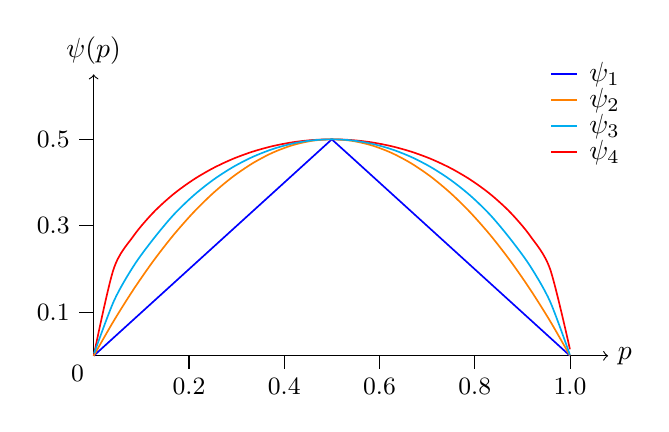
\begin{tikzpicture}[scale=5.5,xscale=1.1]

    \pgfkeys{/pgf/number format/precision=1}

    \draw[<->] (1.08,0) node[right]{$p$} -|(0,0.65) node[above]{$\psi(p)$};
    %\draw[domain=0:1, semithick, smooth, orange] plot ({\x*4},{ln(1/(1-\x))/1.3});
    %\draw[domain=0:1, semithick, cyan] plot ({\x*4},{abs(0-\x)/1.3});

    \draw[domain=0:1,smooth,semithick,red] plot ({\x},{sqrt(\x*(1-\x))});
    \draw[domain=0:1,semithick,blue] plot ({\x},{min(\x,1-\x)});
    \draw[domain=0:1,smooth,semithick,orange] plot ({\x},{2*\x*(1-\x)});
    \draw[domain=0.001:1,smooth,semithick,cyan] plot ({\x},{-\x/2*log2(\x)-(1-\x)/2*log2(1-\x)});

    \node[below left] at (0,0) {\small 0};
    %xticks
    \foreach \x in {0.2,0.4,...,1} {
        \draw (\x,0) -- (\x,-.03);
        \node[below] at (\x,-.03) {\small\pgfmathroundtozerofill{\x}\pgfmathresult};
    }
    \foreach \y in {0.1,0.3,0.5} {
        \draw (0,\y) -- (-.03,\y);
        \node[left] at (-.03,\y) {\small\pgfmathroundtozerofill{\y}\pgfmathresult};
    }
    %legenda
    \foreach \offset/\i/\color in {0/1/blue,0.06/2/orange,0.12/3/cyan,0.18/4/red} {
        \draw [color=\color,thick] (.96,0.65-\offset) -- (.97+.045,0.65-\offset);
        \node[right] at (1.02,0.65-\offset) {$\psi_{\i}$};
    }

\end{tikzpicture}
\vspace{-.6em}